\documentclass[border=10pt,tikz]{standalone}
\usepackage{tikz}
\usetikzlibrary{positioning,arrows.meta,calc,shadings,fit}

% 3D block style: draws a cuboid with shaded front/top/side faces
\newcommand{\block}[7]{%
  % #1 name, #2 x, #3 y, #4 w, #5 h, #6 fill, #7 label
  \begin{scope}[shift={(#2,#3)}]
    \def\d{0.45}% depth offset
    \fill[#6, opacity=0.55] (0,#5) -- (\d,#5+\d) -- (#4+\d,#5+\d) -- (#4,#5) -- cycle; % top
    \fill[#6, opacity=0.75] (#4,0) -- (#4+\d,\d) -- (#4+\d,#5+\d) -- (#4,#5) -- cycle; % side
    \fill[#6] (0,0) rectangle (#4,#5); % front
    \draw[#6!70!black, line width=0.4pt] (0,0) rectangle (#4,#5);
    \draw[#6!70!black, line width=0.3pt, opacity=0.7]
      (0,#5)--(\d,#5+\d)--(#4+\d,#5+\d)--(#4,#5)
      (#4,0)--(#4+\d,\d)--(#4+\d,#5+\d);
    \node[align=center, font=\footnotesize, text=black] at (#4/2,#5/2) {#7};
    \coordinate (#1-west) at (0,#5/2);
    \coordinate (#1-east) at (#4+\d,#5/2);
    \coordinate (#1-north) at (#4/2,#5+\d);
    \coordinate (#1-south) at (#4/2,0);
    \coordinate (#1-ctr) at (#4/2,#5/2);
  \end{scope}%
}

\begin{document}
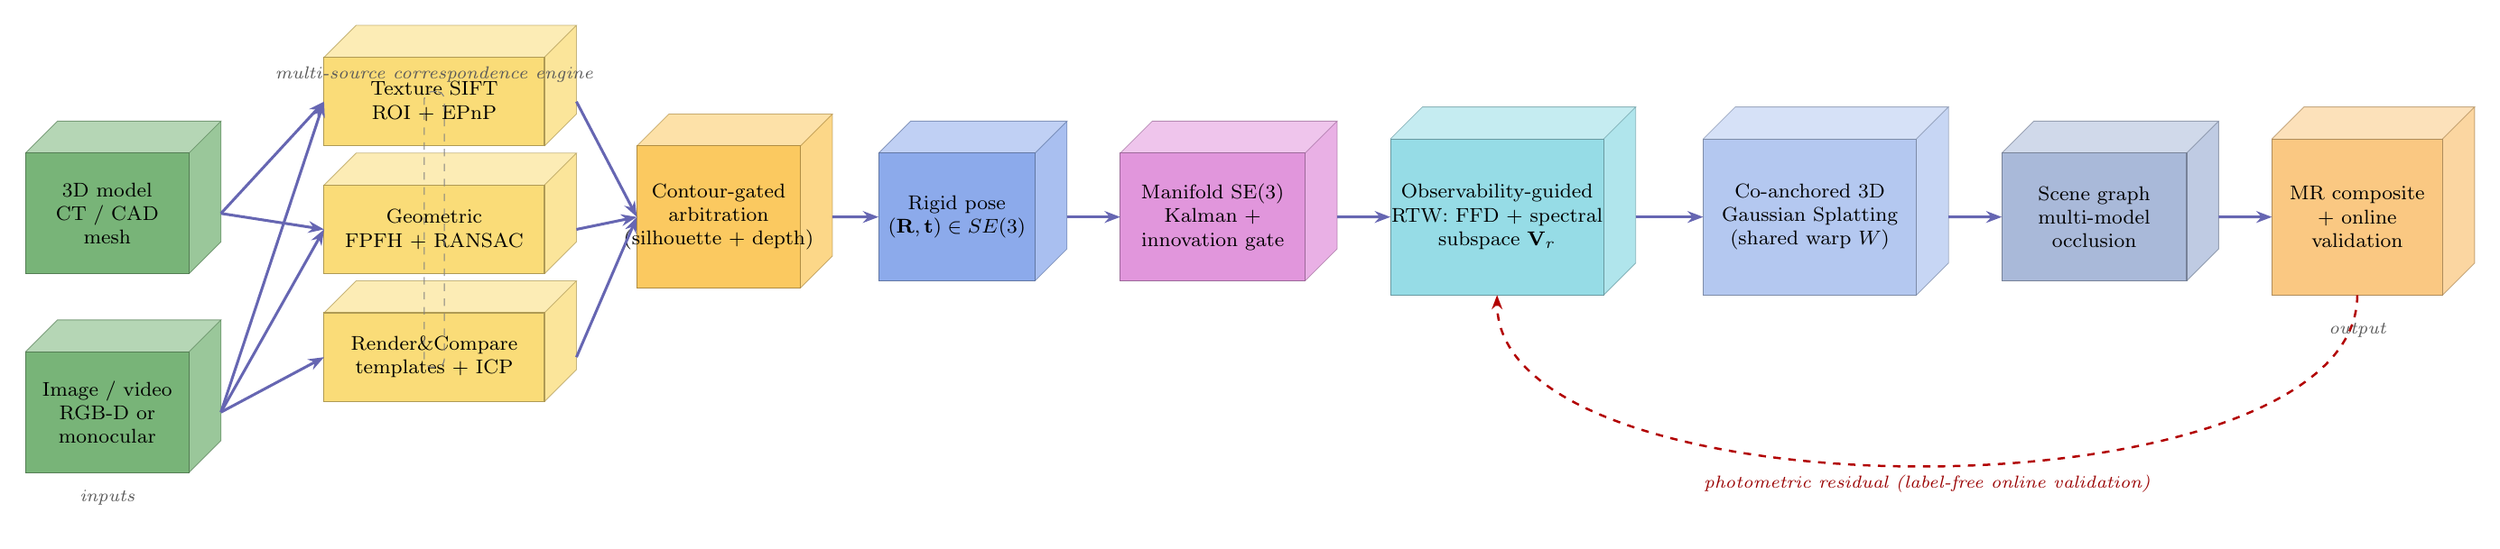
\begin{tikzpicture}[conn/.style={-{Stealth[length=2.2mm]}, line width=1.1pt, draw=blue!50!black!60},
  fb/.style={-{Stealth[length=2mm]}, line width=0.9pt, dashed, draw=red!70!black},
  grp/.style={draw=gray, dashed, rounded corners=3pt, inner sep=4pt},
  glab/.style={font=\scriptsize\itshape, text=gray!70!black}]

\definecolor{incol}{RGB}{120,180,120}
\definecolor{corrcol}{RGB}{250,220,120}
\definecolor{posecol}{RGB}{140,170,235}
\definecolor{kalcol}{RGB}{225,150,220}
\definecolor{rtwcol}{RGB}{150,220,230}
\definecolor{rencol}{RGB}{180,200,240}
\definecolor{outcol}{RGB}{250,200,130}

% ===== INPUTS =====
\block{inmodel}{0}{2.2}{2.3}{1.7}{incol}{3D model\\CT / CAD\\mesh}
\block{inimg}{0}{-0.6}{2.3}{1.7}{incol}{Image / video\\RGB-D or\\monocular}

% ===== CORRESPONDENCE ENGINE (3 branches) =====
\block{csift}{4.2}{4.0}{3.1}{1.25}{corrcol}{Texture SIFT\\ROI + EPnP}
\block{cfpfh}{4.2}{2.2}{3.1}{1.25}{corrcol}{Geometric\\FPFH + RANSAC}
\block{crnc}{4.2}{0.4}{3.1}{1.25}{corrcol}{Render\&Compare\\templates + ICP}
\node[grp, fit=(csift-ctr)(cfpfh-ctr)(crnc-ctr), label={[glab]above:multi-source correspondence engine}] (eng) {};

% ===== ARBITRATION =====
\block{arb}{8.6}{2.0}{2.3}{2.0}{corrcol!80!orange}{Contour-gated\\arbitration\\(silhouette + depth)}

% ===== RIGID POSE =====
\block{pose}{12.0}{2.1}{2.2}{1.8}{posecol}{Rigid pose\\$(\mathbf{R},\mathbf{t})\in SE(3)$}

% ===== KALMAN =====
\block{kal}{15.4}{2.1}{2.6}{1.8}{kalcol}{Manifold SE(3)\\Kalman +\\innovation gate}

% ===== RTW =====
\block{rtw}{19.2}{1.9}{3.0}{2.2}{rtwcol}{Observability-guided\\RTW: FFD + spectral\\subspace $\mathbf{V}_r$}

% ===== RENDERER =====
\block{render}{23.6}{1.9}{3.0}{2.2}{rencol}{Co-anchored 3D\\Gaussian Splatting\\(shared warp $W$)}

% ===== SCENE GRAPH =====
\block{scene}{27.8}{2.1}{2.6}{1.8}{rencol!80!gray}{Scene graph\\multi-model\\occlusion}

% ===== OUTPUT =====
\block{out}{31.6}{1.9}{2.4}{2.2}{outcol}{MR composite\\+ online\\validation}

% ===== CONNECTIONS =====
\draw[conn] (inmodel-east) -- (csift-west);
\draw[conn] (inmodel-east) -- (cfpfh-west);
\draw[conn] (inimg-east)   -- (cfpfh-west);
\draw[conn] (inimg-east)   -- (crnc-west);
\draw[conn] (inimg-east)   -- (csift-west);
\draw[conn] (csift-east) -- (arb-west);
\draw[conn] (cfpfh-east) -- (arb-west);
\draw[conn] (crnc-east)  -- (arb-west);
\draw[conn] (arb-east)   -- (pose-west);
\draw[conn] (pose-east)  -- (kal-west);
\draw[conn] (kal-east)   -- (rtw-west);
\draw[conn] (rtw-east)   -- (render-west);
\draw[conn] (render-east)-- (scene-west);
\draw[conn] (scene-east) -- (out-west);

% validation feedback
\draw[fb] (out-south) .. controls +(0,-3.2) and +(0,-3.2) .. node[midway, below, font=\scriptsize\itshape, text=red!60!black]{photometric residual (label-free online validation)} (rtw-south);

% stage labels
\node[glab] at ($(inimg-south)+(0,-0.35)$) {inputs};
\node[glab] at ($(out-south)+(0,-0.5)$) {output};

\end{tikzpicture}
\end{document}
